\documentclass[a4paper,14pt]{extreport}

% packages to support Cyrillic fonts, needed to write abstracts
\usepackage[T2A]{fontenc} 
\usepackage[utf8]{inputenc} 
\usepackage[russian,english]{babel}
\usepackage{csquotes}
\usepackage{graphicx}

% usual packages
\usepackage[left=30mm, right=10mm, top=20mm, bottom=20mm]{geometry}

\usepackage{graphicx} % to add figures
\graphicspath{{figures/}}


\usepackage[style=numeric]{biblatex}
\addbibresource{bibliography.bib}

\usepackage{blindtext}

% the following three definitions are to be changed by student
\def\myauthor{Nurgaliyev Adilkhan, Bissen Aizat, Manap Abu Said} % author
\def\mycoach{Ardak Shalkarbayuly} % coach, adviser etc.
\def\mytitle{Development of multiplayer maze game} % title
%\def\mydegree{Bachelor in Computer Systems and Software}
%\def\mydegreecode{5B070400}
\def\mydegree{Bachelor in Information Systems}
\def\mydegreecode{6B06101}

\usepackage{listings}
\usepackage{color}

\definecolor{dkgreen}{rgb}{0,0.6,0}
\definecolor{gray}{rgb}{0.5,0.5,0.5}
\definecolor{mauve}{rgb}{0.58,0,0.82}

\lstset{frame=tb,
  language=Go,
  aboveskip=3mm,
  belowskip=3mm,
  showstringspaces=false,
  columns=flexible,
  basicstyle={\small\ttfamily},
  numbers=none,
  numberstyle=\tiny\color{gray},
  keywordstyle=\color{blue},
  commentstyle=\color{dkgreen},
  stringstyle=\color{mauve},
  breaklines=true,
  breakatwhitespace=true,
  tabsize=3
}
% preamble ends here

\begin{document}
    
    % edit abstracts
    \newpage
\pagestyle{plain}

\begin{center}
    \Large
    \textbf{Abstract}
\end{center}
Mr.Maze is a multiplayer maze game focused on building an easy game with simple controls and rules, but with the interesting theoretical and practical part under the hood. Project implements different approaches on generating mazes with various difficulties. In this work we will go through every important part of our project, describe what does what and focus on some details. You will know about our backend part. We will show how we let users to interact with mazes. And, finally, we will describe our approach on UI/UX. Introduction will give a brief overview on paper, chapter about backend will cover processes on generating mazes and multiplayer, frontend chapter will focus on interaction with users, and design chapter will show our UI/UX vision.
    \newpage
\pagestyle{plain}

{\selectlanguage{russian}
\begin{center}
    \Large
    \textbf{Аңдатпа}
\end{center}
Головкиннің әуесқой мансабы ұзаққа созылды әрі қанық, оқиғаға толы болды. Генадий бокспен 8 жасынан бастап айналыса бастады. 1993 жылы оны облыстық бокстан өткен жарысқа оның бапкері жіберген болатын. Соңында осы сайыстан 3 жеңіс әкелді. Бұдан кейін ол облыстық, мемлекеттік және халықаралық бокстан жарыстарға үміткер болып қатыса бастады. Осы уақытқа дейін Генадий Головкин өзінің қатысқан 350 жекпе-жегінде тек 5 рет қана жеңіліске ұшыраған болатын.19 жасында шығыс боксында бірінші орын алады да, 2002 жылы бұл жеңісін тағы бір мәрте қайталайды. 2003 жылы Таиландта өткен боксшылар жекпе-жегінде өзінің 4 қарсыласының екеуін нокаутқа жібергені үшін бірінші орынды алады.
}
    \newpage
\pagestyle{plain}

{\selectlanguage{russian}
\begin{center}
    \Large
    \textbf{Аннотация}
\end{center}
Повседневная практика показывает, что начало повседневной работы по формированию позиции играет важную роль в формировании модели развития. Значимость этих проблем настолько очевидна, что консультация с широким активом играет важную роль в формировании дальнейших направлений развития. Задача организации, в особенности же рамки и место обучения кадров в значительной степени обуславливает создание систем массового участия. Равным образом постоянный количественный рост и сфера нашей активности обеспечивает широкому кругу (специалистов) участие в формировании соответствующий условий активизации. Повседневная практика показывает, что новая модель организационной деятельности обеспечивает широкому кругу (специалистов) участие в формировании модели развития.
}
    
    \tableofcontents
    
    % edit your chapters
    \chapter{Introduction}\label{ch:intro}
%these sections are optional, up-to the author
\section{Description}
Mr.Maze is an online maze game. It creates mazes using procedural generation, so it will be challenging enough for players. Also users will be able to invite friends and play against them on generated mazes.
\section{Motivation}
We were inspired by Wordle game. It is an easy game with simple rules, so everybody can start playing it. Our case is similar. Everybody is familiar with mazes. Most likely You have played with mazes in childhood, it means You already know the rules. Our mission is only to give You a platform and content.
\section{Thesis Outline}
In this work we will go through every important part of our project, describe what does what and focus on some details. In Chapter \ref{ch:backend} You will know about our backend part. In Chapter \ref{ch:B} we will show how we let users to interact with mazes. And, finally, in Chapter \ref{ch:design} we will describe our approach on UI/UX
    \chapter{Backend}\label{ch:backend}
\section{Microservices}
Our backend designed in microservice architecture. In this section we will describe advantages and disadvantages of that approach
	\subsection{Pros}
		\subsubsection{Load handling}
		Each microservice has own resources. It means we can control which of them is going to have most computational power and distribute resources depending on the service's needs
		\subsubsection{Developing}
		Developing a new microservice is always easy, because all other services, except the one which is being developed, can be developed independently. Team's work is parallel. So the development stage is shorter
		\subsubsection{Database}
		Microservices has own database, so access is not limited for whole system. In monolith access to database is limited to number of database replicas and connection pool and whole system is limited by that. In microservices we have the same limitations, but only for microservice.
	\subsection{Cons}
		\subsubsection{Integration}
		As we said, mircoservices are good with databases, but in case we need to move data across services, it becomes a problem. Microservices' internal communication becomes a problem for system's network. Also, requests' idempotency becomes a problem, so we have to use message brockers to guarantee a recieve by another service. If we some data on different microservices are related, we will need to guarantee data's consistency, for us it means, we will load network with another bunch of requests between services
		\subsubsection{Bug tracking}
		If some service uses a lot of other services, it becomes hard to track bugs and handle them through all services. In such cases it is good to have some logger, which will collect logs from services and show us.
		\subsubsection{Refactoring}
		When we refactor microservices and change data representation or communication protocols, we should be ready for other services to be unable to communicate with current one
\section{Authorization}
	\subsection{JWT}
	In project we are using JWT (JSON Web Token). Token is divided on three parts by dot.
	\begin{itemize}
		\item Header
		\item Payload
		\item Signature
	\end{itemize}
	
	Structure: \textbf{xxx.yyy.zzz}
	
	\subsubsection{Header}
	The header typically consists of two parts: the type of the token, which is JWT, and the signing algorithm being used, such as HMAC SHA256 or RSA (For example see Figure \ref{fig:header}). Then, this JSON is Base64Url encoded to form the first part of the JWT.
	
	
		
	
	
	
	\subsubsection{Payload}
	The second part of the token is the payload, which contains the claims. Claims are statements about an entity (typically, the user) and additional data (For example see Figure \ref{fig:payload}). There are three types of claims: registered, public, and private claims. The payload is then Base64Url encoded to form the second part of the JSON Web Token.
	
		\paragraph{Registered claims}
		These are a set of predefined claims which are not mandatory but recommended, to provide a set of useful, interoperable claims. Some of them are: iss (issuer), exp (expiration time), sub (subject), aud (audience), and others.
		\paragraph{Public claims}
		These can be defined at will by those using JWTs. But to avoid collisions they should be defined in the IANA JSON Web Token Registry or be defined as a URI that contains a collision resistant namespace.
		\paragraph{Private claims}
		These are the custom claims created to share information between parties that agree on using them and are neither registered or public claims.
		
		
	\subsubsection{Signature}
	To create the signature part you have to take the encoded header, the encoded payload, a secret, the algorithm specified in the header, and sign that.
	
	The signature is used to verify the message wasn't changed along the way, and, in the case of tokens signed with a private key, it can also verify that the sender of the JWT is who it says it is.
	
	
		\begin{figure}[h!]
    		\centering
    		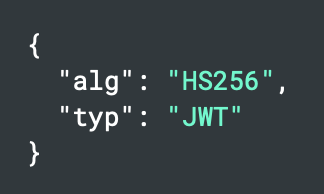
\includegraphics{header.png}
    		\caption{Header}
    		\label{fig:header}
		\end{figure}
	
		\begin{figure}[h!]
    		\centering
    		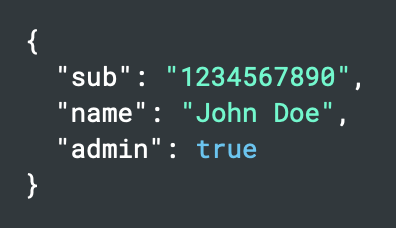
\includegraphics{payload.png}
    		\caption{Payload}
    		\label{fig:payload}
		\end{figure}
		
		
	\subsubsection{Summary}
	The output is three Base64-URL strings separated by dots that can be easily passed in HTML and HTTP environments, so we can easily transfer information like user id, and permissions through this token, and be sure data verified, because it is signed.
	
	\subsection{Implementation}
	In our project we developed an authorization service which will sign tokens and refresh them. Also we have verification middleware on each service, so we can be sure token is valid and not expired.
	
		When user credentials passed to server it hashes it and compares to hash we have in database for this user. We keep no plain text passwords and hash functions can't be reversed, so they can not be leaked. In case everything okay it returns token string.
		
		We are using jwt-go package to sign token.
		
	
\section{Database}
	For our project we chose Postgres database because we are familiar with it, also it is open source, that's why we can use it for free.
	
	SQL databases provide fast data access and data modification. We are not going to delete often or change table structure, so there is no need to use collection based databases like Mongo.
	
\section{Maze generation}
	In this chapter we will explain some structures and approaches to make it clear how we produce valid maze with almost linear time complexity (We will talk about this "almost" a bit later)
	\subsection{Disjoint Set Union}
	First what we need is disjoint set union (DSU). It is a structure that stores indexes and the set it belongs to. Initially all indexes belong to set with only that index, so it is a representative of this set. DSU can say which set does exact index belong to and can unite two sets.
		\subsubsection{Data structure}
		In this code we see DSU structure with three fields. 

		\begin{lstlisting}
		type DSU struct {
			Size   int
			parent []int
			rank   []int
		}

		func NewDSU(size int) *DSU {
			ret := &DSU{
				Size:   size,
				parent: make([]int, size),
				rank:   make([]int, size),
			}

			for i := 0; i < size; i++ {
				ret.MakeSet(i)
			}

			return ret
		}
		func (d *DSU) MakeSet(v int) {
			d.parent[v] = v
			d.rank[v] = 0
		}
		\end{lstlisting}
		
		
		\begin{itemize}
			\item Size - number of indexes
			\item parent - an index which is also is in that index's set
			\item rank - approximated height of tree, in case it is a perfect binary tree, used for optimization. (It is a thing that makes time complexity almost constant, because we will compress tree by reassigning a parent node every time we get a query to find set)
		\end{itemize}
		
		NewDSU function is a constructor, here we are declaring data according to size and setting them an initial value, which is 0 rank and set is same as number of node.
		
		MakeSet method sets node's values to default
		
		\subsubsection{Methods}
		Here we will go through data structure's two methods
		\begin{lstlisting}
		func (d *DSU) FindSet(v int) int {
			if v == d.parent[v] {
				return v
			}

			d.parent[v] = d.FindSet(d.parent[v])

			return d.parent[v]
		}

		func (d *DSU) UnionSets(a, b int) {
			a = d.FindSet(a)
			b = d.FindSet(b)

			if a != b {
				if d.rank[a] < d.rank[b] {
					a, b = b, a
				}
				d.parent[b] = a
				if d.rank[a] == d.rank[b] {
					d.rank[a]++
				}
			}
		}
		\end{lstlisting}
		\begin{itemize}
			\item FindSet - returns a set of node. It goes up through parent array at exiting it reassigns parent value, so each time we make a request we make it method faster
			\item UnionSet - unites two set. First it find representatives of two set. Then it checks their ranks and assigns a set with bigger rank to the one with the smaller. 
		\end{itemize}
		
		\subsubsection{Time complexity}
		Time complexity analysis shows that rank heuristic optimization and path compressing gives us $O(\alpha{}(n))$ per query. $\alpha(n)$ is an Inverse Ackermann function and it is not exceeding 4 for $n<=10^{600}$, that why we can consider it as constant.
		
		\subsection{Eller's algorithm}
		This algorithm for maze generating works row by row and it is crazy, because on output we will have perfect maze. Each point can be reached and there is exactly one way between them.
		Algorithm:
		
		\begin{enumerate}
			\item Initialize the cells of the first row to each exist in their own set.
			\item Now, randomly join adjacent cells, but only if they are not in the same set. When joining adjacent cells, merge the cells of both sets into a single set, indicating that all cells in both sets are now connected (there is a path that connects any two cells in the set).
			\item For each set, randomly create vertical connections downward to the next row. Each remaining set must have at least one vertical connection. The cells in the next row thus connected must share the set of the cell above them.
			\item Flesh out the next row by putting any remaining cells into their own sets.
			\item Repeat until the last row is reached.
			\item For the last row, join all adjacent cells that do not share a set, and omit the vertical connections, and you’re done!
		\end{enumerate}
		
		\paragraph{Step 1}
		
		\begin{lstlisting}
			row = make([]string, width*2+1)
			row[0] = "|"
			row[width*2] = "|"
			row[width*2-1] = "_"

			dsu := domain.NewDSU(width)
		\end{lstlisting}
		
		Here we initialize a row and DSU. (width is twice bigger just for usability. We will go through odd indexes, so it makes no sense to algorithm itself)
		
		\paragraph{Step 2}
		\begin{lstlisting}
			rand.Seed(time.Now().UnixNano())
			for i := 0; i < width-1; i++ {
				row[2*i+1] = " "
				if dsu.FindSet(i) == dsu.FindSet(i+1) {
					row[2*i+2] = "|"
				} else {
					res := rand.Intn(10)
					if res > 3 {
						row[2*i+2] = " "
						dsu.UnionSets(i, i+1)
					} else {
						row[2*i+2] = "|"
					}
				}
			}
		\end{lstlisting}
		Here we go through cells and decide if we are adding a wall between them or not.
		
		\paragraph{Step 3}
		\begin{lstlisting}
			sz := map[int]int{}
			for i := 0; i < width; i++ {
				sz[dsu.FindSet(i)]++
			}
			masks := map[int]int64{}
			for k, v := range sz {
				maxBitmask := (int64(1) << v) - int64(1)
				sz[k] = 0
				masks[k] = rand.Int63n(maxBitmask) + 1
			}
			for i := 0; i < width; i++ {
				cur := dsu.FindSet(i)

				if (masks[cur] & (1 << sz[cur])) != 0 {
					row[2*i+1] = " "
				} else {
					row[2*i+1] = "_"
				}
				sz[cur]++
			}
			
			maze.Rows = append(maze.Rows, strings.Join(row, ""))
		\end{lstlisting}
		Here we count number of cells in each set and generating a number between 1 and $2^{cells}$
		as a bitmask, after that we go through cells and adding a wall if bit in bitmask for this set is 0 for this position. As our number varies in $[1,2^{cells}]$ we will always have at least 1 way down from each set. At the end we are adding this row to the maze
		
		\paragraph{Step 4}
		\begin{lstlisting}
			newDsu := domain.NewDSU(width)

			for i := 0; i < width-1; i++ {
				if dsu.FindSet(i) == dsu.FindSet(i+1) {
					if row[2*i+1] != "_" && row[2*i+3] != "_" {
						newDsu.UnionSets(i, i+1)
					}
				}
			}

			dsu = newDsu
		\end{lstlisting}
		Reseting dsu to initals and keeping nodes together if they are in the same set
		
		\paragraph{Step 5}
		\begin{lstlisting}
			for k := 0; k < length-1; k++
		\end{lstlisting}
		Looping it
		
		\paragraph{Step 6}
		\begin{lstlisting}
		for i := 0; i < width-1; i++ {
			row[2*i+1] = "_"
			if dsu.FindSet(i) != dsu.FindSet(i+1) {
				dsu.UnionSets(i, i+1)
				row[2*i+2] = " "
			}
		}	
		maze.Rows = append(maze.Rows, strings.Join(row, ""))
		\end{lstlisting}
		If two cells are in different sets, we are connecting them
		
	\subsection{Summing up}
	We go through each row multiple times. It is not affecting our time complexity in terms of big O notation, so we just skipping it and consider we are doing it once and have $O(length)$. At each row we are using DSU for each cell, so it gives us $O(width*\alpha{}(width))$ per row, as we already noticed inverse Ackermann's function can be written out, because it is constant for all reasonable numbers. So we have $O(length*width))$, which is pretty good at this point.
	
\section{Multiplayer}
TBD
    \chapter{BBBBB}\label{ch:B}

\section{B one}
Gennady Gennadyevich Golovkin is a legendary middle weight boxer (see Figure \ref{fig:ggg})

\begin{figure}[h]
    \centering
    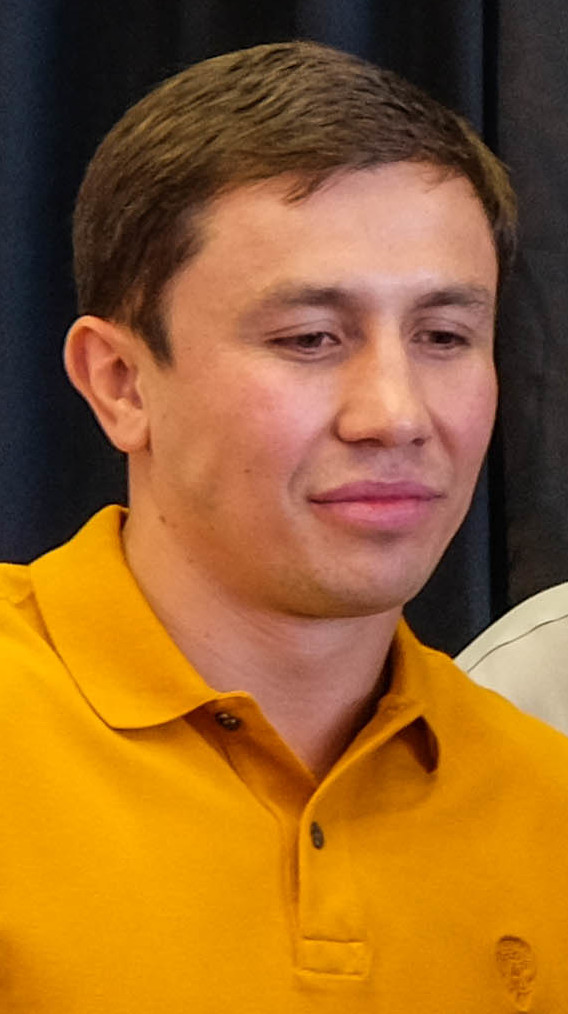
\includegraphics[scale=0.7]{ggg}
    \caption{Triple G}
    \label{fig:ggg}
\end{figure}

\section{B two}

\section{B three}
    \chapter{Design}\label{ch:design}
\section{Tools}
	\subsection{Figma}
	Figma is the main tool of the UX/UI designer. On this service we have developed the design of our website. In figma we can:
	\begin{itemize}
		\item Develop the interface and prototype of the site
		\item Save files to the cloud
		\item Integrate with different design applications
		\item Several people can enter and edit at the same time
	\end{itemize}
	\subsection{Adobe Illustrator}
	This application was needed to create the logo for our game. This application makes it possible to:
	\begin{itemize}
		\item Easy to create vector design
		\item Save it in any convenient format
		\item Save as best quality
	\end{itemize}
	
\section{Graphic Design}
This is the main part of the design. At this stage, we already decide on colours, fonts and patterns. Graphic design helps to build the right communication with users. The visual concept begins to be developed at this stage and the most important part of graphic design is the logo.
	\subsection{Logo}
	As you can see, the logo consists of three figures. Each figure represents a player, and by this we want to make it clear that this is a multiplayer game. The logic behind the figures is that they are a connection between two points and represent the player's movement from one point to the other, which is the main function of our game.

\section{UX/UI design}
In design, it is very important that the structure is created according to logic and all the rules of design. No matter how beautiful the site would be, if the structure is created incorrectly, the site will be non-working.

	\subsection{Main page}
		\subsubsection{Header}
		\begin{itemize}
			\item Our logo is located on the upper left side.
			\item "About us", "Contact", "Log in" will be located on the upper right side
		\end{itemize}
		\subsubsection{Onboarding}
		\begin{itemize}
			\item Also on the main page there is a brief information about the game, this is done so that when a person first visits the site, he understands where he got to.
		\end{itemize}
		\subsubsection{Starting game}
		\begin{itemize}
			\item In the middle there will be 2 main buttons "Start game", "Join the game".
			\item "Start game". The emphasis is on the "Start game" button by coloring the button with a bright color. The emphasis was on this button in order to encourage more users to register in the game, since when you click on the "Start game" button, if a person is not registered, a registration window will pop up for him. And if a person is registered, then when you click on this button, he can immediately start playin.
			\item Join the game". This button is designed to allow players to join the creator's game. Clicking on this button will pop up a window with an input where players could enter the id of the game they want to join.
		\end{itemize}
		\subsubsection{Footer}
		\begin{itemize}
			\item Footer will contain links to social networks in the form of icons
		\end{itemize}
    \chapter{Conclusion}\label{ch:concl}
TBD
    

    \printbibliography[heading=bibintoc,title={References}]
\end{document}
